% arara: clean: {
% arara: --> extensions:
% arara: --> ['aux', 'log', 'out', 'pdf']
% arara: --> }
%! arara: lualatex: {
%! arara: --> shell: yes,
%! arara: --> draft: yes,
%! arara: --> interaction: batchmode
%! arara: --> }
%! arara: biber
% arara: lualatex: {
% arara: --> shell: yes,
% arara: --> draft: no,
% arara: --> interaction: batchmode
% arara: --> }
% arara: lualatex: {
% arara: --> shell: yes,
% arara: --> draft: no,
% arara: --> interaction: batchmode
% arara: --> }
% arara: clean: {
% arara: --> extensions:
% arara: --> ['aux', 'log', 'out']
% arara: --> }
\documentclass[
	12pt,
	oneside,
	appendixprefix=true
]{scrbook}
\usepackage[spanish]{babel}
\decimalpoint
\usepackage{diffcoeff}
\usepackage[intlimits]{mathtools}
\usepackage{amssymb}
\usepackage{amsthm}
\usepackage{graphicx}
\usepackage{minted}
\usepackage[
	citestyle=numeric,
	style=numeric,
	backend=biber,
]{biblatex}
\usepackage{hyperref}

\title{
	Una introducción acerca de los métodos de volúmenes finitos para
	una ecuación de transporte
}
\author{\scshape\name}
\date{\today}

% \addtokomafont{section}{\centering}
% \addtokomafont{subsection}{\centering}

\theoremstyle{definition}
\newtheorem{theorem}{Teorema}
\newtheorem{definition}{Definición}
\newtheorem{remark}{Observación}
\newtheorem{example}{Ejemplo}
\addbibresource{references.bib}

\providecommand{\name}{Carlos Aznarán} % Nombre
\renewcommand{\listingscaption}{Programa}
\renewcommand{\listoflistingscaption}{Lista de \listingscaption s}

\hypersetup{
	pdfencoding=auto,
	linktocpage=true,
	colorlinks=true,
	linkcolor=blue,
	urlcolor=magenta,
	pdfpagelabels,
	pdftex,
	pdfauthor={Carlos Aznarán Laos},
	pdftitle={Una introducción acerca de los métodos de volúmenes
			finitos para una ecuación de transporte},
	pdfsubject={Lecture},
	pdfkeywords={finite volume, pde, transport equation},
	pdfproducer={LuaHBTeX, Version 1.18.0 (TeX Live 2024/Arch Linux)},
	% bookmark=false
}

\clearpage
\pagestyle{empty}
\renewcommand*{\chapterpagestyle}{empty}

\begin{document}

\providecommand{\faculty}{Facultad}
\noindent\parbox[c]{.18\textwidth}{
\includegraphics[width=2.8cm]{logouni}}\hfill
\parbox[c]{1\textwidth}{\raggedright%
    {\large\textbf{UNIVERSIDAD NACIONAL DE INGENIERÍA} \par\smallskip}
    {\large\textbf{\faculty} \par\smallskip}
    {\large\textbf{DEPARTAMENTO ACADÉMICO DE CIENCIAS BÁSICAS} \par\smallskip}
}

\begin{center}\bfseries\large
    Práctica Dirigida 5 de Métodos Numéricos (BMA-18)
\end{center}

\vspace{-0.5cm}

\hrulefill
\vspace{-2.5mm}

\rule{16.5cm}{0.8mm}

\section{Semana 8}

\subsection{Métodos de Runge-Kutta}

En esta sección analizamos los métodos basados en evaluaciones de
$f\left(x,y\right)$ en puntos intermedios del intervalo
$\left[x_{n},x_{n+1}\right]$ de modo que resulten métodos
equivalentes a un método de Taylor de cierto orden.
Así, de forma más precisa, un método tipo Runge-Kutta basado en
$m$-evaluaciones se describe como sigue:

Dada una partición del intervalo $\left[a,b\right]$ donde existe
solución del P.V.I. en $N$-subintervalos, se define la solución
numérica, $\left\{y_n\right\}_{n=0,\ldots,N}$ siguiente:
\begin{equation}\label{eq:rungekutta}
    \begin{aligned}
        y_{0}   & =\mu                                                       \\
        y_{n+1} & =y_{n}+h\sum_{j=1}^{m}b_{j}K_{j}, \quad n=0,1, \ldots, N-1
    \end{aligned}
\end{equation}
donde
\begin{equation*}
    K_{i}\left(x,y\right)=
    f\left(x+c_{i}h,y+h\sum_{j=1}^m a_{i j}K_{j}\left(x,y\right)\right) \quad i=1, \ldots, m
\end{equation*}

Observando la expresión de las $K^{\prime}$ s es evidente que se requiere de algunas aclaraciones:
\begin{itemize}
    \item
          El método descrito es, en general, IMPLÍCTO;
    \item
          El método es EXPLÍCITO si $a_{i j}=0$ para $j \geq i$;
    \item
          Para $a_{i j}=0$ para $j>i$ es método se dice DIAGONALMENTE IMPLÍCITO.
    \item
          El método es CONSISTENTE si, y sólo si, $\sum_{i=1}^m b_i=1$
    \item
          Un método~\eqref{eq:rungekutta} puede representarse mediante el llamado arreglo de Butcher siguiente:
          \begin{table}[ht!]
              \centering
              \begin{tabular}{c|ccc}
                  $c_1$    & $a_{11}$  & $\cdots$ & $a_{1 m}$ \\
                  $\vdots$ & $\vdots$  & $\ddots$ & $\vdots$  \\
                  $c_m$    & $a_{m 1}$ & $\cdots$ & $a_{m m}$ \\
                  \hline   & $b_1$     & $\cdots$ & $b_m$
              \end{tabular}
          \end{table}
\end{itemize}
Además, en orden a simplificar el análisis de estos métodos se suponen las igualdades siguientes:
\begin{equation}\label{eq:coefficients}
    c_i=\sum_{j=1}^m a_{i j} \quad i=1, \ldots, m
\end{equation}

Nos centraremos en el análisis de los métodos Runge-Kutta EXPLÍCITOS, es decir, las constantes se describen por:
\begin{align*}
    K_1 & =f(x, y)                                                                \\
    K_i & =f\left(x+c_i h, y+h \sum_{j=1}^{i-1} a_{i j} K_j\right) i=2, \ldots, m
\end{align*}

\subsubsection{Métodos de dos evaluaciones explícitos}

Teniendo en cuenta las condiciones de consistencia y~\eqref{eq:coefficients}
para los métodos~\eqref{eq:rungekutta} podemos escribir el de dos evaluaciones en la forma:
\begin{equation}\label{eq:twosteps}
    \begin{aligned}
        y_0     & =\mu                                                                   \\
        y_{n+1} & =y_n+h\left((1-\alpha) K_1+\alpha K_2\right), \quad n=0,1, \ldots, N-1
    \end{aligned}
\end{equation}
donde
\begin{align*}
    K_1 & =f\left(x_n, y_n\right)                     \\
    K_2 & =f\left(x_n+\beta h, y_n+h \beta K_1\right)
\end{align*}

Así, analizando el error de truncatura local, podemos deducir el
orden máximo del método y sus distintas opciones.

A tal fin aplicamos sendos desarrollos de Taylor para la solución del
P.V.I. y para la función $f\left(x,y\right)$ respecto de ambas
variables.
Más precisamente,
\begin{equation*}
    R_{n+1}\left(x\right)=
    y\left(x+h\right)-y\left(x\right)-h\left((1-\alpha) K_1+\alpha K_2\right)
\end{equation*}
donde
\begin{equation*}
    K_{1}=f(x, y(x));\quad K_2=f(x+\beta h, y(x)+h \beta f(x, y(x)))
\end{equation*}
que desarrollando en el punto $(x, y(x))$ tenemos (notamos $y=y(x), f=f(x, y), \ldots$ ):
\begin{align*}
    K_2 & =f(x+\beta h, y+h \beta f)=T_2(f ; \beta h, \beta h f)+O\left(h^3\right)= \\
        & =f+\beta h F+\frac{\beta^2 h^2}{2} G+O\left(h^3\right)
\end{align*}
Por lo tanto, tendremos que:
\begin{align*}
    R_{n+1}(x) & =h y^{\prime}+\frac{h^2}{2} y^{\prime \prime}+\frac{h^3}{6} y^{\prime \prime \prime}+O\left(h^4\right)-h\left[(1-\alpha) f+\alpha\left(f+\beta h F+\frac{\beta^2 h^2}{2} G+O\left(h^3\right)\right)\right]= \\
               & =h^2\left(\frac{1}{2}-\alpha \beta\right) F+h^3\left(\frac{1}{6} y^{\prime \prime \prime}-\frac{\alpha \beta^2}{2} G\right)+O\left(h^4\right)=                                                              \\
               & =h^2\left(\frac{1}{2}-\alpha \beta\right) F+\frac{h^3}{6}\left[\left(1-3 \alpha \beta^2\right) G+f_y \cdot F\right]+O\left(h^4\right)
\end{align*}
es decir, el método~\eqref{eq:twosteps} es de orden 2 si el coeficiente en $h^2$ es cero; a saber,
\begin{equation*}
    \alpha \beta=\frac{1}{2}
\end{equation*}

% Esta igualdad conduce a una familia de métodos RK de orden 2. En particular,
% - para $\alpha=1 \Rightarrow \beta=\frac{1}{2}$, se obtiene el método (2.8)
% - para $\alpha=\frac{1}{2} \Rightarrow \beta=1$, se obtiene el método (2.9)

\subsubsection{Método explícito de 4 evaluaciones (Runge-Kutta clásico)}

Este es un método de orden 4 que se describe como sigue:
\begin{align*}
    y_0     & =\mu                                                                      \\
    y_{n+1} & =y_n+\frac{h}{6}\left(K_1+2 K_2+2 K_3+K_4\right) \quad n=0,1, \ldots, N-1
\end{align*}
donde
\begin{align*}
    K_1 & =f\left(x_n, y_n\right)                 \\
    K_2 & =f\left(x_n+h / 2, y_n+h / 2 K_1\right) \\
    K_3 & =f\left(x_n+h / 2, y_n+h / 2 K_2\right) \\
    K_4 & =f\left(x_n+h, y_n+h K_3\right)
\end{align*}
El orden del método se obtiene mediante desarrollos de Taylor adecuados en cada $K_i$ como puede apreciarse en el siguiente proceso (simplificado):
\begin{align*}
    K_2 & =T_3\left(f ; \frac{h}{2}, \frac{h}{2} f\right)+O\left(h^4\right)=f+\frac{h}{2} F+\frac{h^2}{8} G+\frac{h^3}{48} H+O\left(h^4\right)                                                                               \\
    K_3 & =T_3\left(f ; \frac{h}{2}, \frac{h}{2} K_2\right)+O\left(h^4\right)=f+\frac{h}{2} D_{\left(1, K_2\right)} f+\frac{h^2}{8} D_{\left(1, K_2\right)}^2 f+\frac{h^3}{48} D_{\left(1, K_2\right)}^3 f+O\left(h^4\right) \\
    K_4 & =T_3\left(f ; h, h K_3\right)+O\left(h^4\right)=f+h D_{\left(1, K_3\right)} f+\frac{h^2}{2} D_{\left(1, K_3\right)}^2 f+\frac{h^3}{6} D_{\left(1, K_3\right)}^3 f+O\left(h^4\right)
\end{align*}
podemos escribir:
\begin{align*}
    D_{\left(1, K_2\right)} f   & =F+\frac{h}{2} f_y F+\frac{h^2}{8} f_y G+O\left(h^3\right)                                                                                          \\
    D_{\left(1, K_2\right)}^2 f & =G+h F\left(f_{x y}+f \cdot f_{y y}\right)+O\left(h^2\right)                                                                                        \\
    D_{\left(1, K_2\right)}^3 f & =H+O(h)                                                                                                                                             \\
    \Rightarrow K_3             & =f+\frac{h}{2} F+\frac{h^2}{8}\left(G+2 f_y F\right)+\frac{h^3}{48}\left[H+3 f_y G+6\left(f_{x y}+f \cdot f_{y y}\right) F\right]+O\left(h^4\right)
\end{align*}
de forma análoga:
\begin{align*}
    D_{\left(1, K_3\right)} f   & =F+\frac{h}{2} f_y F+\frac{h^2}{8} f_y\left(G+2 F f_y\right)+O\left(h^3\right)                                                                                 \\
    D_{\left(1, K_3\right)}^2 f & =G+h F\left(f_{x y}+f \cdot f_{y y}\right)+O\left(h^2\right)                                                                                                   \\
    D_{\left(1, K_3\right)}^3 f & =H+O(h)
    \Rightarrow K_4             & =f+h F+\frac{h^2}{2}\left(G+f_y F\right)+\frac{h^3}{48}\left[8 H+24\left(f_{x y}+f \cdot f_{y y}\right) F+6 f_y\left(G+2 f_y F\right)\right]+O\left(h^4\right)
\end{align*}

por lo tanto
\begin{equation*}
    \frac{K_1+2 K_2+2 K_3+K_4}{6}=f+\frac{h}{2} F+\frac{h^2}{6}\left(G+f_y F\right)+\frac{h^3}{24}\left(H+f_y G+F\left(f_y^2+3 f_{x y}+3 f \cdot f_{y y}\right)\right)+O\left(h^4\right)
\end{equation*}
De todo lo anterior se obtiene el error de truncatura local del método:
\begin{align*}
    R_{n+1}(x)= & h y^{\prime}+\frac{h^2}{2} y^{\prime \prime}+\frac{h^3}{6} y^{\prime \prime \prime}+\frac{h^4}{24} y^{i v)}+O\left(h^5\right)-h \frac{K_1+2 K_2+2 K_3+K_4}{6}= \\
    =           & h\left(y^{\prime}-f\right)+\frac{h^2}{2}\left(y^{\prime \prime}-F\right)+\frac{h^3}{6}\left(y^{\prime \prime \prime}-\left(G+f_y F\right)\right)+              \\
                & +\frac{h^4}{24}\left(y^{i v)}-\left(H+f_y G+F\left(f_y^2+3 f_{x y}+3 f \cdot f_{y y}\right)\right)\right)+O\left(h^5\right)
\end{align*}

\subsection{Método de Euler}

El método de Euler consiste en encontrar iterativamente la solución
de una ecuación diferencial de primer orden y valores iniciales
conocidos para un rango de valores. Partiendo de un valor inicial
$x_0$ y avanzando con un paso $h$, se pueden obtener los valores de
la solución de la siguiente manera:
\begin{equation*}
    Y_{k+1}=Y_k+h \cdot f\left(x_k, Y_k\right)
\end{equation*}
Donde $Y$ es solución de la ecuación diferencial y $f$ es la ecuación
diferencial en función de las variables independientes.

\begin{questions}
    \question

    Se quiere obtener el valor de la corriente en el siguiente circuito RL hasta un segundo con un paso de un cuarto de segundo:

    \begin{figure}[ht!]
        \centering
        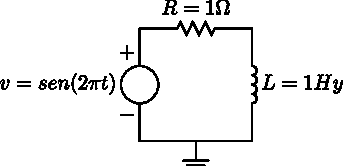
\includegraphics[width=.4\paperwidth]{circuit}
    \end{figure}

    Planteando la malla correspondiente se puede obtener la ecuación del circuito de la figura:

    \begin{align*}
        v                     & =R \cdot i(t)+L \cdot \frac{\mathrm{~d} i(t)}{\mathrm{dt}} \\
        \operatorname{sen}(t) & =i(t)+i^{\prime}(t)                                        \\
        i^{\prime}(t)         & =\operatorname{sen}(2 \pi t)-i(t)=f(t, i)
    \end{align*}
    Reescribiendo la fórmula de iteración con nuestras variables del problema llegamos a:
    \begin{equation*}
        I_{k+1}=I_k+h \cdot f\left(t_k, I_k\right)
    \end{equation*}
    En primer lugar, reconocemos nuestros datos iniciales como $t_0=0$ e $I_0=0$.
    Además, la función será, en este caso, la derivada de la corriente. Respecto a $t_k$, dado que hay un paso constante $h$, se puede observar que en general $t_k=t_0+h \cdot k$; por lo tanto, se puede observar que tomará tres iteraciones llegar a $t=1$ debido a que los valores de salida siempre están un paso adelantado. Según nuestros índices, la primer iteración será la número $0$:
    \begin{align*}
        k=0 &                                     \\
            & I_1=I_0+h \cdot f(0 ; 0)=0          \\
        k=1 &                                     \\
            & I_2=I_1+h \cdot f(0,25 ; 0)=0,25    \\
        k=2 &                                     \\
            & I_3=I_2+h \cdot f(0,5 ; 1)=0,1875   \\
        k=3 &                                     \\
            & I_4=I_3+h \cdot f(0,75 ;-1)=-0,1093
    \end{align*}
    La solución de la ecuación diferencial, teóricamente, es:
    \begin{equation*}
        i(t)=\frac{1}{1+4 \pi^2} \cdot\left(2 \pi e^{-t}+\operatorname{sen}(2 \pi t)-2 \pi \cos (2 \pi t)\right)
    \end{equation*}
    Comparando con los valores teóricos:
    \begin{table}[ht!]
        \centering
        \begin{tabular}{|c|c|c|c|}
            \hline$t$ & Valor teórico & Valor aproximado & Error  \\
            \hline 0  & 0             & 0                & 0      \\
            0,25      & 0,1455        & 0                & 0,1455 \\
            0,5       & 0,2493        & 0,25             & 0,0007 \\
            0,75      & 0,0486        & 0,1875           & 0,1389 \\
            1         & $-0,0981$     & $-0,1093$        & 0,0112 \\
            \hline
        \end{tabular}
    \end{table}
    Para mejorar la aproximación, se puede aumentar el tamaño de puntos (es decir, reducir el tamaño del paso $h$ ).
    Por otro lado, se puede utilizar un método de mayor orden para obtener una mejor aproximación usando la misma cantidad de puntos.
\end{questions}

\subsection{Método de Heun}

Este método consiste en una mejora del método de Euler para resolver ecuaciones
diferenciales de primer orden y conocido el valor inicial.
En este caso, lo que se realiza es un promedio entre el valor obtenido por
Euler y otro obtenido a partir de la aproximación del valor de la función en el punto siguiente, también por Euler.
\begin{equation*}
    Y_{k+1}=Y_k+\frac{h}{2}\left[f\left(x_k, Y_k\right)+f\left(x_{k+1}, Y_{k+1}^{\cdot}\right)\right]
\end{equation*}
Donde $Y$ es solución de la ecuación diferencial, $f$ es la ecuación diferencial en función de las
variables independientes y la solución de $Y_{k+1}^*$ es una aproximación de Euler.

\begin{questions}
    \question
    Recordando la ecuación diferencial del ejercicio anterior:
    \begin{equation*}
        i^{\prime}(t)=\operatorname{sen}(2 \pi t)-i(t)=f(t, i)
    \end{equation*}
    Obtenemos la fórmula de iteración según el método de Heun:

    \begin{equation*}
        I_{k+1}=I_k+\frac{h}{2}\left[f\left(t_k, I_k\right)+f\left(t_{k+1}, I_{k+1}\right)\right]
    \end{equation*}
    Nuevamente, los valores iniciales son $t_0=0, I_0=0$.
    En este caso, definiremos un valor $I_{k+1}^{\dot{~}}$ que corresponde a la
    aproximación de Euler en el paso siguiente.
    Realizando los cálculos:
    \begin{align*}
         & k=0                                                                                           \\
         & \dot{I}_1=I_0+h \cdot f(0 ; 0)=0                                                              \\
         & I_1=I_0+\frac{h}{2}\left[f(0 ; 0)+f\left(0,25 ; \dot{I}_1\right)\right]=0,125=i(0,25)         \\
         & k=1                                                                                           \\
         & \dot{I}_2=I_1+h \cdot f(0,25 ; 0,125)=0,3437                                                  \\
         & I_2=I_1+\frac{h}{2}\left[f(0,25 ; 0,125)+f\left(0,5 ; \dot{I}_2\right)\right]=0,1914=i(0,5)   \\
         & k=2                                                                                           \\
         & \dot{I}_3=I_2+h \cdot f(0,5 ; 0,1914)=0,1435                                                  \\
         & I_3=I_2+\frac{h}{2}\left[f(0,5 ; 0,1914)+f\left(0,75 ; \dot{I}_3\right)\right]=0,0245=i(0,75) \\
         & k=3                                                                                           \\
         & \dot{I}_4=I_3+h \cdot f(0,75 ; 0,0245)=-0,2316                                                \\
         & I_4=I_3+\frac{h}{2}\left[f(0,75 ; 0,245)+f\left(0,75 ; \dot{I}_4\right)\right]=-0,0745=i(1)
    \end{align*}

    Comparando con los valores teóricos:
    \begin{table}[ht!]
        \centering
        \begin{tabular}{|c|c|c|c|}
            \hline$t$ & Valor teórico & Valor aproximado & Error   \\
            \hline 0  & 0             & 0                & 0       \\
            0,25      & 0,1455        & 0,125            & 0,00205 \\
            0,5       & 0,2493        & 0,1914           & 0,0579  \\
            0,75      & 0,0486        & 0,0245           & 0,00241 \\
            1         & $-0,0981$     & $-0,0745$        & 0,00242 \\
            \hline
        \end{tabular}
    \end{table}

    A continuación, se ilustran la solución en un gráfico que relaciona la curva esperada
    con los puntos obtenidos por el método de Heun y de Euler:
    \begin{figure}[ht!]
        \centering
        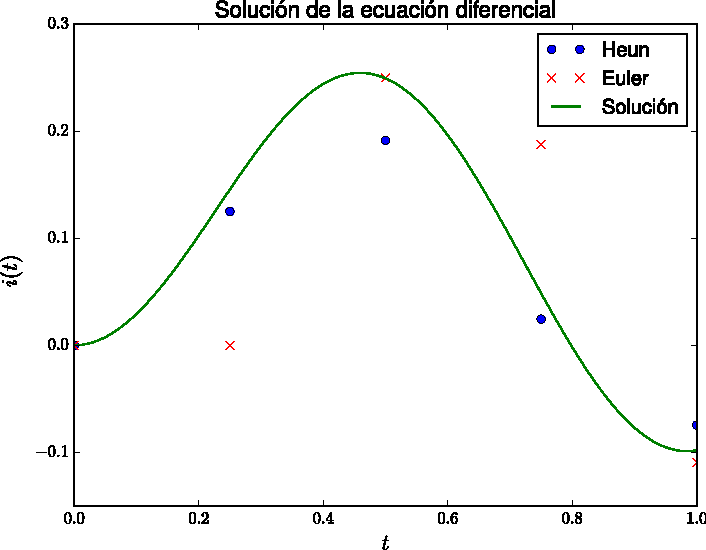
\includegraphics[width=.4\paperwidth]{solutionheun}
    \end{figure}
    Se puede observar que, si bien para ciertos puntos el comportamiento es mejor para Euler, para el
    método de Heun, los puntos se comportan mejor según la forma de la solución respecto a la solución
    de Euler.
\end{questions}

\subsection{Derivación e integración numérica}

\begin{questions}
    \question

    Calcular usando la fórmula del punto medio:
    \begin{equation*}
        \int_a^b f(x) \dl x \cong(b-a) f\left(\frac{a+b}{2}\right).
    \end{equation*}
    La integral
    \begin{equation*}
        \int_0^1 x \dl x.
    \end{equation*}
    Calcular la integral exacta y dar el error. Dibujar el área exacta y aproximada y explicar el error.

    \question

    Usando la regla del trapecio compuesta con tres subintervalos, calcular:
    \begin{equation*}
        \int_0^1 x^2 \dl x.
    \end{equation*}
    Calcular la integral exacta y el error. Hacer un dibujo del área exacta y la aproximada.

    \question

    Usando la regla de Simpson calcular:
    \begin{equation*}
        \int_0^1 x^3 \dl x.
    \end{equation*}
    Calcular la integral exacta y calcular el error. ¿Qué curva utiliza para aproximar la función la regla de Simpson? ¿Cómo explicarías el error?

    \question

    Dada la integral:
    \begin{equation*}
        \int_{-\infty}^{\infty} e^{-x^2} \dl x=\sqrt{\pi} \approx 1,77245.
    \end{equation*}
    Aproximar la integral de forma que el resultado sea exacto hasta las décimas, usando la fórmula de los trapecios compuesta ¿Cuántos subintervalos son necesarios? (Indicación: se puede tomar un intervalo menor que $(-\infty, \infty)$, por ejemplo $[-2,2])$

    \question

    Supongamos que la fórmula de la integración numérica
    \begin{equation*}
        \int_{-2}^2 f(x) \dl x \simeq A_0 f(-1)+A_1 f(0)+A_2 f(1)
    \end{equation*}
    es de tipo interpolatorio.
    Determinar los coeficientes (pesos) de la fórmula utilizando las condiciones del grado de precisión. ¿Cuál es el grado de precisión de dicha fórmula? Razónese la respuesta. Calcular la integral si $f(x)=\cosh x$. ¿Con qué curva crees que hemos interpolado la función para aproximar su integral?

    \question

    Calcular los nodos y los pesos de la fórmula de Newton-Cotes abierta con dos nodos para el intervalo $[-1,1]$.
    Determinar su grado de precisión. Calcular la integral si $f(x)=$ cosh $x$.
    ¿Con qué curva crees que hemos interpolado la función para aproximar su integral?

    \question

    \begin{parts}
        \part


        Obtener $x_0$ para la fórmula de cuadratura
        \begin{equation*}
            \int_{-1}^1 f(x) \dl x \simeq 2 f\left(x_0\right)
        \end{equation*}
        tenga grado de precisión al menos uno. ¿Cuál es su grado de precisión?

        \part

        Obtener $x_0 y x_1$ para que la fórmula de cuadratura
        \begin{equation*}
            \int_{-1}^1 f(x) \dl x \simeq f\left(x_0\right)+f\left(x_1\right)
        \end{equation*}
        tenga grado de precisión al menos dos. ¿Cuál es su grado de precisión? ¿Es de Newton-Cotes?

        \part
        Usar la fórmula obtenida anteriormente para calcular un valor aproximado de:
        \begin{equation*}
            \int_{-2}^2\left(x^2+1\right) \dl x
        \end{equation*}
        realizando previamente un cambio de variable adecuado.
        ¿Qué error se comete al aplicar dicha fórmula en este ejercicio?
        Justificar la respuesta sin hacer la integral exacta.
    \end{parts}

    \question

    \begin{parts}
        \part


        Aproximar mediante las reglas del trapecio y de Simpson el valor de la integral
        \begin{equation*}
            I=\int_0^3\left(x^3+1\right) \dl x.
        \end{equation*}

        \part

        Comparar los valores aproximados con el valor exacto. ¿Se podría haber predicho alguno de los errores?

        \part

        Utilizando la regla de los trapecios compuesta para aproximar $I$,
        ¿qué número de subintervalos será suficiente para que el error, en valor absoluto, sea menor que $10^{-6}$ ?
    \end{parts}

    \question

    Sea la integral:
    \begin{equation*}
        I=\int_0^1 e^{-x^2} \dl x.
    \end{equation*}

    \begin{parts}
        \part
        Obtener el valor aproximado de la integral mediante la regla del trapecio compuesta con dos subintervalos. Acotar el error en valor absoluto usando la fórmula del error.

        \part

        Determinar el número $n$ de subintervalos de modo que la regla del trapecio compuesta aproxime el valor de $I$ con un error menor que $10^{-6}$.
    \end{parts}

    \question

    Es conocido que
    \begin{equation*}
        \log 2=\int_1^2 \frac{1}{x} \dl x
    \end{equation*}
    y damos como dato que si $f$ tiene derivada cuarta continua en $\left[a,b\right]$
    entonces el error de la fórmula de Simpson compuesta viene dado por:
    \begin{equation*}
        E_h^S=
        -\frac{(b-a) h^4}{180} f^{(4)}(c), \quad c \in(a, b)
    \end{equation*}

    \begin{parts}
        \part
        Aproximar el valor de $\log 2$ mediante la fórmula de Simpson compuesta que utiliza dos subintervalos (es decir, cinco nodos) y acotar el error en valor absoluto usando la fórmula del error. Comparar esta cota con el error verdadero.

        \part

        Determinar el número total de nodos que serán suficientes para que la fórmula de Simpson compuesta proporcione un valor aproximado de $\log 2$ con un error menor que $10^{-4}$.
    \end{parts}

    \question

    Si se utiliza la regla de los trapecios compuesta para aproximar:
    \begin{equation*}
        I=\int_1^2 \ln ^2(x) \dl x
    \end{equation*}
    ¿Qué número de subintervalos será suficiente elegir para que el error fuese menor que $10^{-3}$ ?

    \question

    \begin{parts}
        \part
        Encontrar las constantes $A_0$, $A_1$, $x_1$ de modo que la fórmula de cuadratura simple:
        \begin{equation*}
            \int_{0}^{1}f(x)\dl x \simeq A_0f(0)+A_1f(x_1)
        \end{equation*}
        tenga el grado de precisión más alto posible. ¿Cuál es el grado de precisión? ¿Es una fórmula de Newton-Cotes?

        \part
        Realizar un cambio de variable en la integral
        \begin{equation*}
            \int_{0}^{2}(1+e^{-x^2})\dl x
        \end{equation*}
        para poder utilizar la fórmula obtenida anteriormente y calcular de esta manera una aproximación del valor de dicha integral.
    \end{parts}
\end{questions}


%\subsection{Solución numérica de sistemas de ecuaciones diferenciales ordinarias con condiciones iniciales y de ecuaciones diferenciales ordinarias de orden superior}

\providecommand{\name}{Nombre}
\vfill{Nombre}\footnote{Hecho en \LaTeX}
\hfill{UNI, 3 de marzo de 2025}

\end{document}